\documentclass[12pt,a4paper]{article}

% ---------- Idioma y codificación ----------
\usepackage[utf8]{inputenc}
\usepackage[T1]{fontenc}
\usepackage{mathpazo}
% Si tu distribución no tiene instalado el idioma español, esta línea evita
% que la compilación falle (instalá "babel-spanish" para tenerlo completo).
\IfFileExists{spanish.ldf}
  {\usepackage[spanish,es-nodecimaldot,es-noshorthands]{babel}}
  {\usepackage[english]{babel}}
% Nota: la opción es-noshorthands (arriba) desactiva los shorthands "<" y ">"
% de babel-spanish, que de otro modo rompen la sintaxis de flechas de TikZ
% (">={...}").

% ---------- Página ----------
\usepackage[a4paper,top=3cm,bottom=2.5cm,left=2.5cm,right=2.5cm,headheight=1.5cm,headsep=0.8cm]{geometry}

% ---------- Utilidades ----------
\usepackage{graphicx}
\usepackage{fancyhdr}
\usepackage{lastpage}          % necesario para \pageref{LastPage}
\usepackage{xcolor}
\usepackage{enumitem}
\usepackage{tikz}
\usetikzlibrary{positioning,shapes.geometric,arrows.meta,calc,fit,backgrounds}
\usepackage[hidelinks]{hyperref}
\usepackage{titlesec}
\usepackage{float}
\usepackage{booktabs}
\usepackage{longtable}
\usepackage{amsmath}
\usepackage{amssymb}
\usepackage{listings}
\usepackage[numbers]{natbib}
\bibliographystyle{unsrtnat}
\newcommand{\sectionbreak}{\clearpage}

% ---------- Estilo para código Verilog ----------
\definecolor{codegray}{gray}{0.96}
\definecolor{codekw}{RGB}{0,90,160}
\definecolor{codecom}{RGB}{100,120,100}
\definecolor{codestr}{RGB}{160,60,60}
\definecolor{codenum}{gray}{0.45}

\lstdefinestyle{verilog}{
  language=Verilog,
  backgroundcolor=\color{codegray},
  basicstyle=\ttfamily\scriptsize,
  keywordstyle=\color{codekw}\bfseries,
  commentstyle=\color{codecom}\itshape,
  stringstyle=\color{codestr},
  numbers=left,
  numberstyle=\tiny\color{codenum},
  numbersep=8pt,
  showstringspaces=false,
  breaklines=true,
  breakatwhitespace=true,
  frame=single,
  rulecolor=\color{gray!40},
  framesep=4pt,
  xleftmargin=16pt,
  tabsize=4,
  captionpos=b,
  columns=fullflexible,
  morekeywords={always,posedge,negedge,localparam,parameter,logic,endcase,
                signed,unsigned,task,endtask,function,endfunction,initial,
                integer,timescale,display,finish,random,time,clog2,signed}
}
\lstset{style=verilog}
\renewcommand{\lstlistingname}{Código}

% ============================================================
%  >>>>>>>>>>  DATOS DEL TRABAJO: EDITAR ACÁ  <<<<<<<<<<
% ============================================================
\newcommand{\Titulo}{Trabajo Práctico N°2: UART}
\newcommand{\Subtitulo}{Maquinas de Estado Finitas: UART}
\newcommand{\Materia}{Arquitectura de Computadoras}
\newcommand{\Institucion}{Facultad de Ciencias Exactas, Físicas y Naturales - Universidad Nacional de Córdoba}
\newcommand{\Carrera}{Ingeniería en Computación}
%\newcommand{\Fecha}{\today}

% Integrantes: una línea \persona{...} por cada uno
\newcommand{\Integrantes}{%
  \persona{Brigido, Tomás Andrés}{Legajo 38481096}%
  \persona{Tosolini, Agustín}{Legajo 42332698}%
}

% Docentes
\newcommand{\Docentes}{%
  \persona{Pereyra, Martin}{}%
}

% Repositorio: dejar vacío {} para que NO aparezca en la carátula
\newcommand{\Repositorio}{https://github.com/Agustin-Tosolini/Computer-Architecture-FCEFyN/tree/main/Laboratories/Lab2}

% Logos del encabezado
\newcommand{\LogoIzquierdo}{./logos/unc.png}
\newcommand{\LogoDerecho}{./logos/fcefyn.png}
\newcommand{\AlturaLogo}{3.0cm}
% ============================================================


% ---------- Maquinaria interna (no hace falta tocar) ----------
\newcommand{\ponerlogo}[1]{%
  \IfFileExists{#1}{%
    \includegraphics[height=\AlturaLogo,keepaspectratio]{#1}%
  }{%
    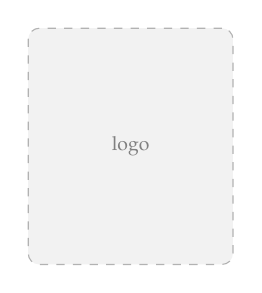
\begin{tikzpicture}
      \node[draw=gray!60,dashed,fill=gray!10,rounded corners,
            minimum height=\AlturaLogo,minimum width=2.6cm,
            font=\scriptsize\color{gray}] {logo};
    \end{tikzpicture}%
  }%
}

% Estilo de la carátula: sin encabezado (los logos van dentro de la página)
\fancypagestyle{caratula}{%
  \fancyhf{}
  \renewcommand{\headrulewidth}{0pt}
  \renewcommand{\footrulewidth}{0pt}
}

% Resto del documento: sólo el número de página al pie, SIN logos
\fancypagestyle{plain}{%
  \fancyhf{}
  \fancyfoot[C]{\small Página \thepage\ de \pageref{LastPage}}
  \renewcommand{\headrulewidth}{0pt}
  \renewcommand{\footrulewidth}{0pt}
}
\pagestyle{plain}

\newcommand{\persona}[2]{%
  \textbf{#1}%
  \ifx\relax#2\relax\else{\ \small(#2)}\fi\\[0.25em]
}

\setlength{\emergencystretch}{3em}
\hyphenpenalty=1000
\setlength{\parskip}{0.6em}
\setlength{\parindent}{0pt}

% ---------- Estilos de TikZ para los diagramas ----------
\tikzset{
  bloque/.style   = {draw, rounded corners, align=center, font=\small,
                     minimum width=2.8cm, minimum height=1.3cm},
  estado/.style   = {draw, rounded corners, align=center, font=\small,
                     minimum width=3.2cm, minimum height=0.9cm},
  salida/.style   = {draw, rounded corners, align=center, font=\small,
                     minimum width=3.2cm, minimum height=1.3cm},
  etiqueta/.style = {font=\scriptsize, align=left},
  flecha/.style   = {-{Stealth[length=2mm]}}
}


% ============================================================
\begin{document}

% ------------------------- CARÁTULA -------------------------
\thispagestyle{caratula}
\begin{center}
  % --- Logos: aparecen únicamente en esta página
  \noindent\makebox[\textwidth]{%
    \ponerlogo{\LogoIzquierdo}\hfill\ponerlogo{\LogoDerecho}%
  }\\[0.35cm]
  \rule{\textwidth}{0.4pt}

  \vspace{0.5cm}

  {\large \Institucion \par}
  {\normalsize \Carrera \par}

  \vspace{0.5cm}
  \rule{\textwidth}{1.2pt}\\[0.6cm]
  {\Huge\bfseries \Titulo \par}
  \vspace{0.3cm}
  \ifx\Subtitulo\empty\else{\Large \Subtitulo \par}\vspace{0.3cm}\fi
  \rule{\textwidth}{1.2pt}

  \vspace{0.7cm}
  {\large \textit{\Materia} \par}

  \vspace{0.75cm}
  {\large\bfseries Integrantes\par}
  \vspace{0.4cm}
  \Integrantes

  \vspace{1cm}
  {\large\bfseries Docente\par}
  \vspace{0.4cm}
  \Docentes

  \vspace{1cm}
  {\large\bfseries Repositorio\par}
  \vspace{0.4cm}
  \Repositorio

  \vfill

  %{\large \Fecha \par}
  \vspace{1cm}
\end{center}

\newpage

% --------------------- ÍNDICE ---------------------
\tableofcontents
\newpage

% ============================================================
\section{Introducción}
% ============================================================

El objetivo de este trabajo práctico es diseñar e implementar en Verilog una
UART (\emph{Universal Asynchronous Receiver and Transmitter}) y utilizarla para
comunicar la ALU desarrollada en el trabajo práctico anterior con una
computadora.

El sistema funciona bajo un esquema de pregunta y respuesta: la PC envía por el
puerto serie tres bytes (el operando A, el operando B y el código de operación),
la FPGA los recibe, la ALU calcula el resultado y este vuelve a la PC como un
único byte. Las banderas de la ALU (\emph{zero}, \emph{carry} y
\emph{overflow}) se muestran en los LEDs de la placa.

El trabajo se apoya casi por completo en máquinas de estado finitas: el
receptor, el transmisor y el control del protocolo son tres máquinas
independientes que se coordinan entre sí mediante señales de \emph{handshake}.

\subsection{Herramientas utilizadas}

\begin{itemize}[nosep]
  \item \textbf{Lenguaje:} Verilog (únicamente).
  \item \textbf{Síntesis e implementación:} Vivado 2026.1.
  \item \textbf{Placa:} Digilent Basys 3 (Artix-7 XC7A35T-1CPG236C, reloj de 100~MHz).
  \item \textbf{Verificación:} simulación funcional con dos \emph{testbenches} propios.
  \item \textbf{Prueba sobre la placa:} script de Python con interfaz gráfica
        (Tkinter y \texttt{pyserial}) que envía los operandos y verifica el
        resultado contra un modelo de la ALU escrito en Python.
\end{itemize}

% ============================================================
\section{Marco teórico}
% ============================================================

\subsection{Máquinas de estado finitas}

Una máquina de estado finita (FSM) modela un sistema que en cada instante se
encuentra en \emph{un único} estado de un conjunto finito, y que evoluciona
según la secuencia de entradas que recibe. Son la herramienta natural para
problemas en los que la acción a tomar depende de lo que ocurrió antes, y no
solo de la entrada actual.

Según de qué dependan las salidas se distinguen dos tipos:

\begin{itemize}[nosep]
  \item \textbf{Moore:} la salida depende únicamente del estado actual. Como
        proviene directamente de registros, no presenta \emph{glitches}.
  \item \textbf{Mealy:} la salida depende del estado y de la entrada. Suele
        requerir menos estados, pero la salida puede cambiar entre flancos de
        reloj.
\end{itemize}

En este trabajo el receptor y el transmisor se implementaron como máquinas de
Moore, ya que sus salidas van a la línea serie o son pulsos de aviso que deben
ser limpios. El control del protocolo se implementó como Mealy, porque sus
salidas (\texttt{rd} y \texttt{wr}) son señales internas que deben activarse en
el mismo ciclo en que se consume o entrega un dato.

\subsubsection{FSMD}

Una FSM pura codifica toda su memoria en el registro de estado. Si el receptor
se modelara así, necesitaría un estado distinto por cada combinación de
``cuántos ticks pasaron'', ``cuántos bits llegaron'' y ``qué bits llegaron'',
lo que daría una cantidad inmanejable de estados.

La solución es separar el problema en dos partes, lo que se conoce como
\textbf{FSMD} (\emph{FSM with Datapath}):

\begin{itemize}[nosep]
  \item la \textbf{FSM} decide \emph{qué hacer} y recuerda solo la fase
        (\texttt{IDLE}, \texttt{START}, \texttt{DATA}, \ldots);
  \item el \textbf{datapath} son registros auxiliares (contadores y registros de
        desplazamiento) que guardan \emph{cuánto} y \emph{con qué} se está
        trabajando.
\end{itemize}

Gracias a esta separación, el receptor se resuelve con cinco estados en lugar de
miles.

\subsubsection{Codificación de estados}

Los estados se codificaron con \textbf{one-hot}, es decir un bit por estado, que
es la codificación recomendada en FPGA: la lógica de decodificación se reduce a
mirar un solo bit, lo que favorece la frecuencia máxima. Todas las máquinas
incluyen una rama \texttt{default} que, ante una codificación inválida, devuelve
la máquina a su estado inicial (máquina de estado segura).

\subsection{Comunicación serie asíncrona}

En una comunicación \emph{asíncrona} no existe una línea de reloj compartida
entre emisor y receptor. Ambos extremos solo acuerdan de antemano la
\textbf{velocidad} en baudios, es decir la duración de cada bit. A 9600 baudios
cada bit dura $1/9600 \approx 104{,}17\,\mu$s.

La información viaja agrupada en tramas con la siguiente estructura:

\begin{table}[H]
  \centering
  \small
  \begin{tabular}{@{}lll@{}}
    \toprule
    \textbf{Campo} & \textbf{Duración} & \textbf{Valor} \\
    \midrule
    Línea en reposo & indefinida & 1 \\
    Bit de start    & 1 bit      & 0 \\
    Bits de datos   & 8 bits     & el byte, LSB primero \\
    Bit de stop     & 1 bit      & 1 \\
    \bottomrule
  \end{tabular}
  \caption{Trama utilizada en este trabajo (8-N-1).}
\end{table}

El bit de start es el que permite al receptor sincronizarse: su flanco de bajada
marca el comienzo de la trama. A partir de ahí el receptor mide el tiempo por su
cuenta, contando con su propio reloj.

\subsubsection{Sobremuestreo 16x}

Como el receptor solo conoce el flanco inicial, necesita una forma de ubicarse
en el \emph{centro} de cada bit, que es donde la señal está estable. Para eso se
divide cada bit en 16 intervalos iguales, llamados \emph{ticks}. Contando 8
ticks desde el flanco de start el receptor queda en el medio del bit de start, y
a partir de ahí cada 16 ticks cae en el centro de cada bit de datos.

El factor 16 es interno del receptor: no se transmite ni el emisor lo conoce.
Además del alineamiento, el sobremuestreo aporta tolerancia frente a la
diferencia de frecuencia entre los relojes de ambos extremos.

% ============================================================
\section{Arquitectura del sistema}
% ============================================================

El diseño se organizó en tres bloques, siguiendo el diagrama de bloques
propuesto en la consigna.

\begin{figure}[H]
  \centering
  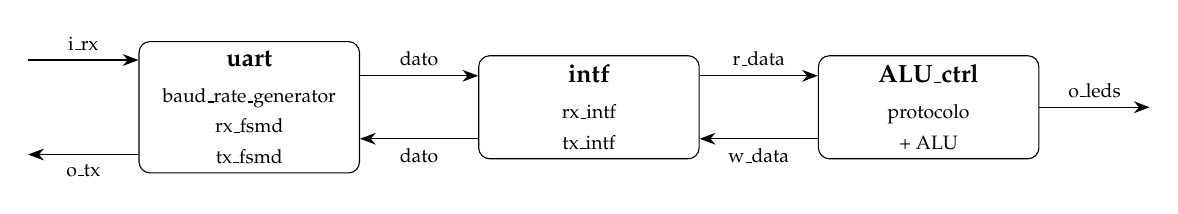
\begin{tikzpicture}[node distance=1.6cm and 1.5cm]
    \node[bloque] (uart) {\textbf{uart}\\[2pt]\scriptsize baud\_rate\_generator\\\scriptsize rx\_fsmd\\\scriptsize tx\_fsmd};
    \node[bloque, right=of uart] (intf) {\textbf{intf}\\[2pt]\scriptsize rx\_intf\\\scriptsize tx\_intf};
    \node[bloque, right=of intf] (ctrl) {\textbf{ALU\_ctrl}\\[2pt]\scriptsize protocolo\\\scriptsize + ALU};

    \draw[flecha] ([yshift=4mm]uart.east) -- node[etiqueta, above]{dato} ([yshift=4mm]intf.west);
    \draw[flecha] ([yshift=-4mm]intf.west) -- node[etiqueta, below]{dato} ([yshift=-4mm]uart.east);

    \draw[flecha] ([yshift=4mm]intf.east) -- node[etiqueta, above]{r\_data} ([yshift=4mm]ctrl.west);
    \draw[flecha] ([yshift=-4mm]ctrl.west) -- node[etiqueta, below]{w\_data} ([yshift=-4mm]intf.east);

    \draw[flecha] ([yshift=6mm]uart.west) ++(-1.4cm,0) -- node[etiqueta, above]{i\_rx} ([yshift=6mm]uart.west);
    \draw[flecha] ([yshift=-6mm]uart.west) -- node[etiqueta, below]{o\_tx} ++(-1.4cm,0);
    \draw[flecha] (ctrl.east) -- node[etiqueta, above]{o\_leds} ++(1.4cm,0);
  \end{tikzpicture}
  \caption{Bloques principales del sistema.}
\end{figure}

\begin{table}[H]
  \centering
  \small
  \begin{tabular}{@{}lll@{}}
    \toprule
    \textbf{Módulo} & \textbf{Tipo} & \textbf{Función} \\
    \midrule
    \texttt{uart\_alu\_top}        & top       & instancia los tres bloques, expone los pines \\
    \texttt{uart}                  & wrapper   & agrupa el generador y las dos FSMD \\
    \texttt{baud\_rate\_generator} & contador  & genera el tick de sobremuestreo \\
    \texttt{rx\_fsmd}              & FSMD      & recibe una trama y entrega un byte \\
    \texttt{tx\_fsmd}              & FSMD      & transmite un byte como trama \\
    \texttt{intf}                  & wrapper   & agrupa los dos buffers \\
    \texttt{rx\_intf}              & buffer    & guarda el byte recibido, bandera \texttt{rx\_empty} \\
    \texttt{tx\_intf}              & buffer    & bandera \texttt{tx\_full} y pulso de arranque \\
    \texttt{ALU\_ctrl}             & FSM       & protocolo de tres bytes y registros A, B, opcode \\
    \texttt{ALU}                   & combinacional & operaciones aritméticas y lógicas \\
    \bottomrule
  \end{tabular}
  \caption{Módulos del diseño.}
\end{table}

El criterio de separación fue que cada módulo tenga una única responsabilidad y
una interfaz angosta. En particular, la UART no sabe qué significan los bytes
que mueve, y el módulo \texttt{ALU\_ctrl} es el único que conoce el protocolo.
La ALU quedó como lógica puramente combinacional, sin reloj ni registros, tal
como fue escrita en el trabajo práctico anterior, cambiando únicamente quién le
entrega los operandos.

% ============================================================
\section{Generador de baud rate}
% ============================================================

Es un contador módulo $N$ que emite un pulso de \emph{un solo ciclo} de reloj
cada $N$ ciclos. Es importante destacar que \textbf{no es un reloj}: es una
señal de habilitación (\emph{enable}) que se usa como condición dentro de los
bloques secuenciales. Utilizarla como reloj generaría un reloj derivado de
lógica combinacional, algo desaconsejado en FPGA porque no utiliza la red
dedicada de distribución de reloj y complica el análisis de tiempos.

El divisor se calcula como:

\begin{equation}
  N = \frac{f_{clk}}{\text{BaudRate} \times 16}
  = \frac{100{\times}10^{6}}{9600 \times 16} = 651{,}04 \approx 651
\end{equation}

\begin{table}[H]
  \centering
  \small
  \begin{tabular}{@{}rrrr@{}}
    \toprule
    \textbf{Baudios} & \textbf{$N$} & \textbf{Bits del contador} & \textbf{Error} \\
    \midrule
    9600   & 651 & 10 & $+0{,}006\%$ \\
    19200  & 326 & 9  & $-0{,}147\%$ \\
    38400  & 163 & 8  & $-0{,}147\%$ \\
    115200 & 54  & 6  & $+0{,}47\%$ \\
    \bottomrule
  \end{tabular}
  \caption{Divisor y error para distintas velocidades con reloj de 100~MHz.}
\end{table}

Se eligió 9600 baudios porque el redondeo del divisor introduce el menor error
de todas las opciones y la velocidad es más que suficiente para transmitir tres
bytes por operación. El ancho del contador se calcula automáticamente con
\texttt{\$clog2}, de modo que al cambiar la velocidad no haya que ajustarlo a
mano.

\begin{lstlisting}[caption={Generador de baud rate.}]
localparam integer N     = CLK_FREQ / (BAUD_RATE * OVERSAMP);
localparam integer WIDTH = $clog2(N);

reg [WIDTH-1:0] counter = {WIDTH{1'b0}};

always @(posedge i_clk) begin
    if (i_reset)              counter <= {WIDTH{1'b0}};
    else if (counter == N-1)  counter <= {WIDTH{1'b0}};
    else                      counter <= counter + 1'b1;
end

assign o_tick = (counter == N-1);
\end{lstlisting}

La salida se decodifica directamente del registro (\emph{output equals state}),
por lo que el pulso de un ciclo se obtiene sin lógica adicional.

% ============================================================
\section{Receptor}
% ============================================================

\subsection{Máquina de estados (\texttt{rx\_fsmd})}

El receptor es una FSMD con cinco estados. Su datapath está formado por tres
registros:

\begin{itemize}[nosep]
  \item \texttt{s}: cuenta los ticks dentro del bit actual (0 a 15).
  \item \texttt{n}: cuenta los bits de datos ya recibidos.
  \item \texttt{b}: registro de desplazamiento donde se arma el byte.
\end{itemize}

\begin{figure}[H]
    \centering
    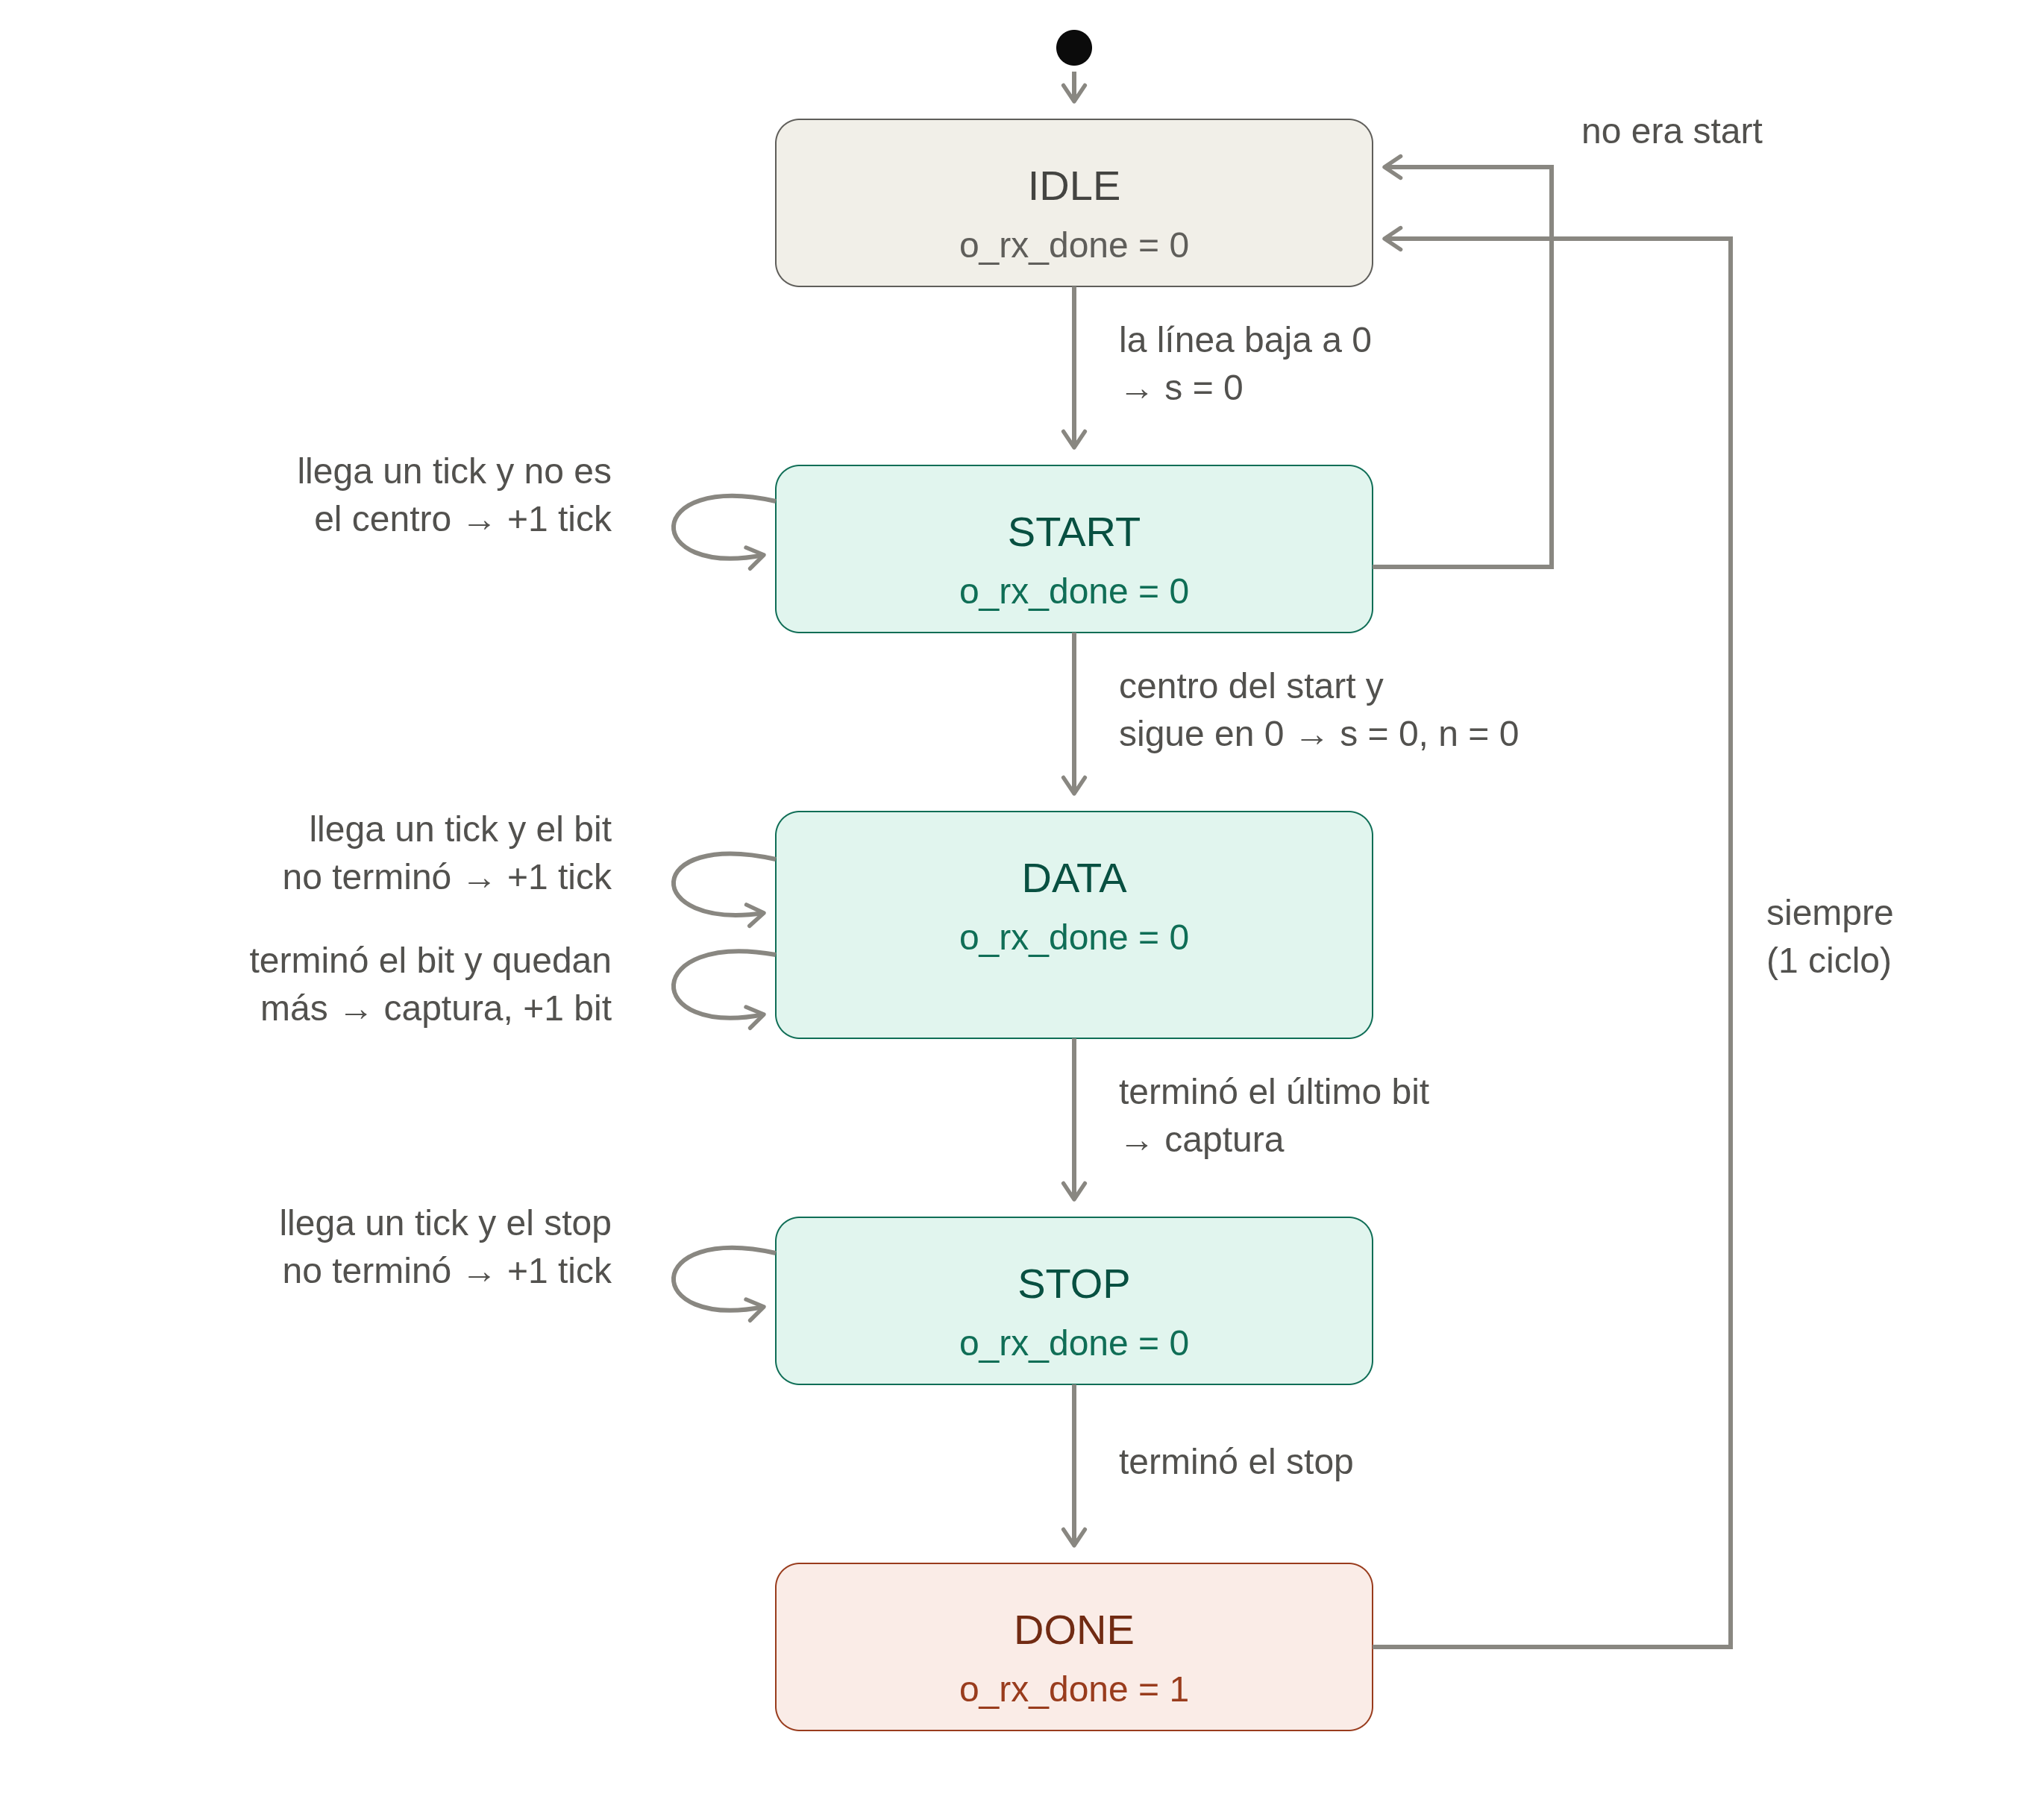
\includegraphics[width=\textwidth]{img/diagrama_estados_rx_fsmd.png}
    \caption{Diagrama de estados del receptor (máquina de Moore).}
    \label{fig:state-diagram-rx}
\end{figure}

El funcionamiento estado por estado es el siguiente:

\begin{itemize}[nosep]
  \item \textbf{IDLE:} observa la línea en cada ciclo de reloj (no espera al
        tick, para no llegar tarde al flanco). Cuando la línea baja a 0,
        comienza una trama.
  \item \textbf{START:} cuenta 8 ticks, es decir medio bit, para ubicarse en el
        centro del bit de start. Si en ese punto la línea volvió a 1, lo que
        bajó fue ruido y la máquina regresa a \texttt{IDLE}.
  \item \textbf{DATA:} cada 16 ticks cae en el centro de un bit, lo muestrea y
        lo ingresa al registro de desplazamiento. Como UART transmite el LSB
        primero, el bit nuevo entra por la izquierda y el registro se desplaza a
        la derecha, de modo que al recibir los ocho bits el byte queda ordenado.
  \item \textbf{STOP:} espera un bit completo desde el centro del último dato,
        con lo cual termina en el centro del bit de stop.
  \item \textbf{DONE:} dura un solo ciclo y es el único estado donde
        \texttt{o\_rx\_done} vale 1. Existe para que ese aviso sea una salida de
        Moore.
\end{itemize}

\begin{lstlisting}[caption={Estado DATA del receptor.}]
DATA:
    if (i_s_tick) begin
        if (s == 15) begin
            s_next = {S_BITS{1'b0}};
            b_next = {rx_sync, b[DATA_BITS-1:1]};
            if (n == DATA_BITS-1)
                next_state = STOP;
            else
                n_next = n + 1'b1;
        end
        else
            s_next = s + 1'b1;
    end
\end{lstlisting}

\subsubsection{Sincronizador de entrada}

La línea \texttt{i\_rx} proviene de la PC y no guarda ninguna relación con el
reloj de la FPGA, por lo que sus flancos pueden caer justo sobre un flanco de
reloj y dejar un flip-flop en estado metaestable. Para evitarlo, la señal pasa
por dos flip-flops en cascada antes de entrar a la lógica: el primero absorbe el
riesgo y el segundo, un ciclo después, entrega un valor ya estable que todos los
registros de la máquina leen por igual. Ambos se inicializan en 1, que es el
valor de reposo de la línea, para no detectar un bit de start falso al encender
la placa.

\subsubsection{Elección del punto de muestreo}

Una decisión de diseño importante fue terminar el estado \texttt{STOP} en el
\emph{centro} del bit de stop y no en su final. De esta manera queda medio bit
de margen antes de que pueda comenzar la trama siguiente, lo que absorbe la
diferencia de frecuencia acumulada entre los dos relojes a lo largo de la trama.
En las simulaciones se verificó que con este criterio el receptor tolera
desvíos de hasta un 3\% con tramas consecutivas sin pausa.

\subsection{Interface del receptor (\texttt{rx\_intf})}

La FSMD muestra el byte recibido durante un único ciclo, junto con el pulso
\texttt{o\_rx\_done}, y vuelve inmediatamente a esperar la trama siguiente. Esa
ventana es demasiado angosta para el resto del sistema, de modo que el interface
guarda el dato y levanta una bandera que se mantiene hasta que alguien lo
consuma.

\begin{lstlisting}[caption={Lógica del buffer de recepción.}]
wire accept = i_rx_done && (!full || i_rd);

always @(posedge i_clk) begin
    if (i_reset)     full <= 1'b0;
    else if (accept) full <= 1'b1;   // entro un byte
    else if (i_rd)   full <= 1'b0;   // lo consumieron
end

assign o_r_data   = buffer;
assign o_rx_empty = ~full;
\end{lstlisting}

La condición \texttt{accept} contempla el caso en que llega un byte nuevo en el
mismo ciclo en que el consumidor lee el anterior, de modo que no se pierde
ningún dato.

% ============================================================
\section{Transmisor}
% ============================================================

\subsection{Máquina de estados (\texttt{tx\_fsmd})}

Para el transmisor se optó por armar la \textbf{trama completa} en un único
registro de desplazamiento al momento de recibir el pedido, en lugar de generar
cada campo desde un estado distinto. Como start, datos y stop pasan a ser
simplemente ``un bit más de la trama'', la máquina se reduce a tres estados.

La trama se arma con la concatenación \texttt{\{stop, dato, start\}}: en Verilog
lo que se escribe a la izquierda ocupa los bits más significativos, por lo que el
bit de start queda en la posición 0 y es el primero en salir.

\begin{figure}[H]
    \centering
    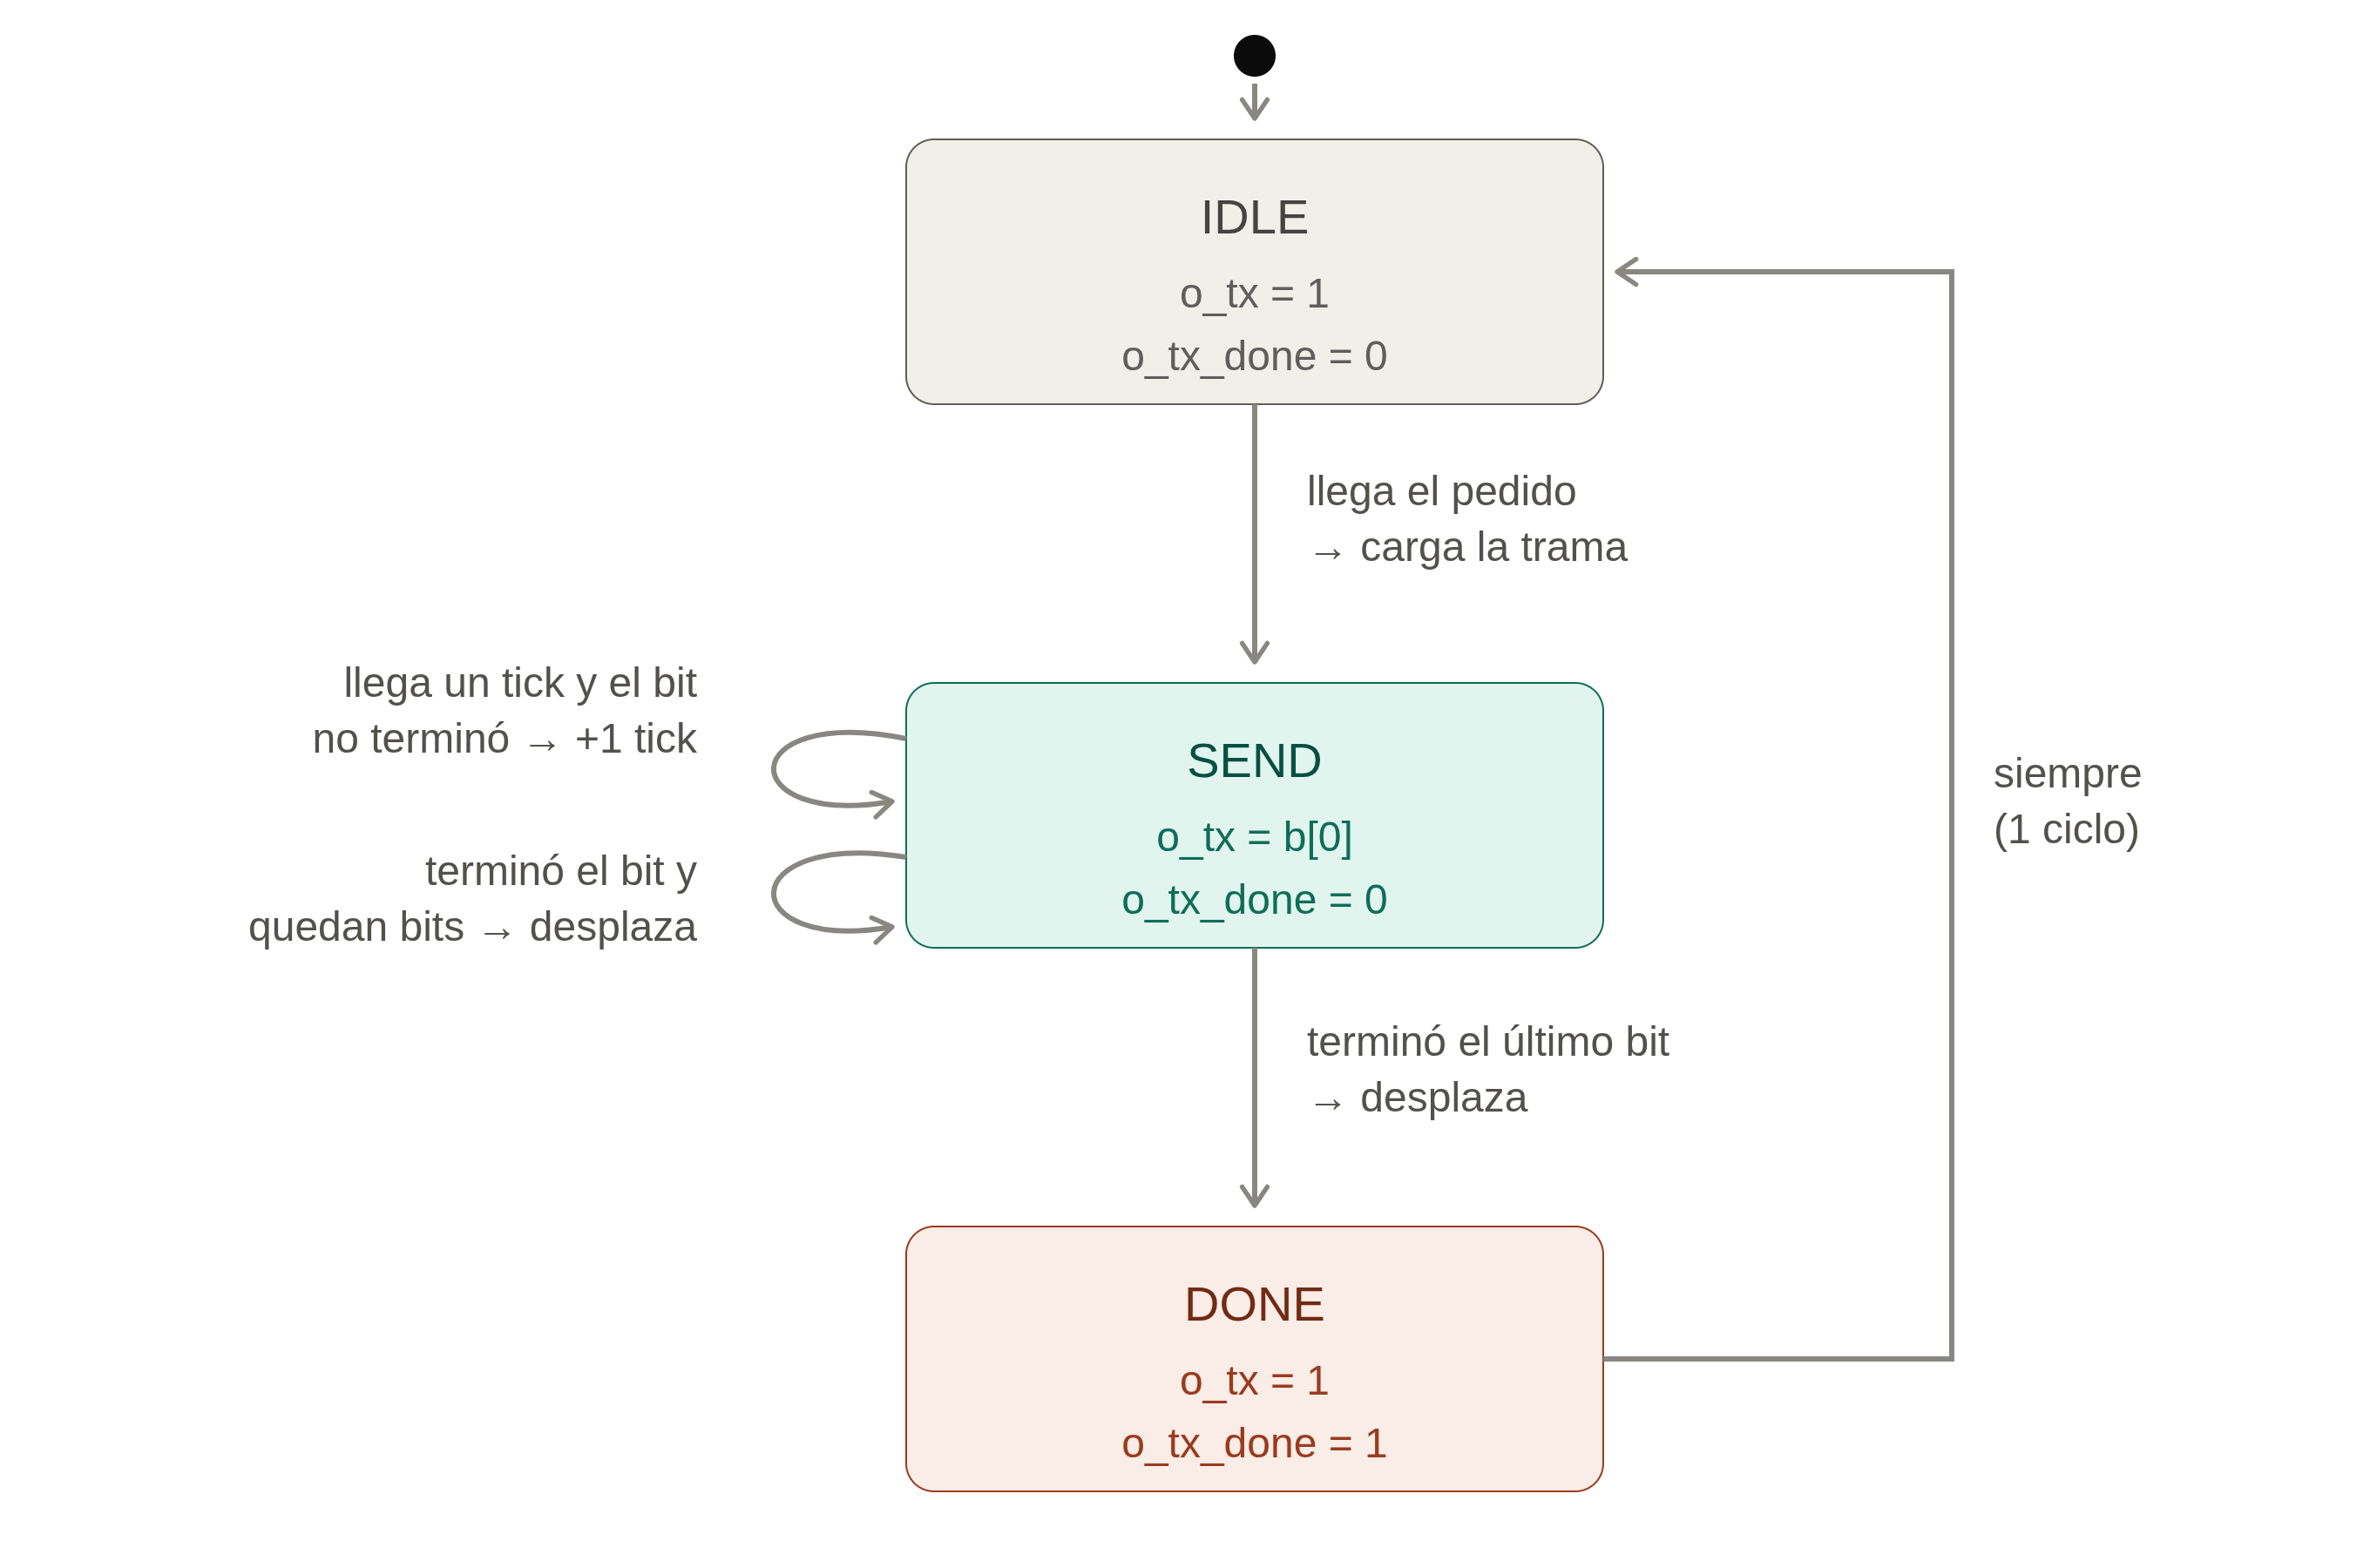
\includegraphics[width=\textwidth]{img/diagrama_estados_tx_fsmd.png}
    \caption{Diagrama de estados del transmisor (máquina de Moore).}
    \label{fig:state-diagram-tx}
\end{figure}

\newpage

\begin{lstlisting}[caption={Carga de la trama y desplazamiento.}]
IDLE:
    if (i_tx_start) begin
        b_next     = {{STOP_BITS{STOP_BIT}}, i_din, START_BIT};
        s_next     = {S_BITS{1'b0}};
        n_next     = {N_BITS{1'b0}};
        next_state = SEND;
    end

SEND:
    if (i_s_tick) begin
        if (s == 15) begin
            s_next = {S_BITS{1'b0}};
            b_next = {1'b1, b[FRAME_BITS-1:1]};
            ...
\end{lstlisting}

Al desplazar se introducen unos por la izquierda, de modo que cuando la trama
termina de salir el registro queda en todos unos y la línea vuelve sola al
estado de reposo. La salida es directamente un bit del registro
(\texttt{o\_tx~=~b[0]}), sin lógica intermedia, lo que garantiza una señal libre
de \emph{glitches}: esto es importante porque la línea sale del chip hacia un
receptor asincrónico, que podría interpretar un pulso espurio como un bit de
start.

Una diferencia con el receptor es que el estado \texttt{START} no existe como
tal y que la trama se transmite completa, incluyendo el bit de stop entero: el
transmisor debe garantizar la duración que promete, mientras que al receptor le
conviene cortar antes para ganar margen.

\subsection{Interface del transmisor (\texttt{tx\_intf})}

A diferencia del interface de recepción, este no necesita guardar el dato,
porque la FSMD lo copia a su propio registro en el mismo ciclo en que recibe el
pedido. Lo único que almacena es \emph{estado}: si hay una transmisión en curso.

\begin{lstlisting}[caption={Bandera de ocupado del transmisor.}]
always @(posedge i_clk) begin
    if (i_reset)            full <= 1'b0;
    else if (i_wr && !full) full <= 1'b1;   // arranca una transmision
    else if (i_tx_done)     full <= 1'b0;   // el tx_fsmd termino
end

assign o_tx_start = i_wr && !full;
assign o_tx_din   = i_w_data;
assign o_tx_full  = full;
\end{lstlisting}

La bandera cumple dos funciones con una sola señal: le informa al control si
puede escribir y, a la vez, impide que se genere un pulso de arranque mientras
el transmisor está ocupado. Esto último es necesario porque la FSMD solo atiende
el pedido cuando se encuentra en \texttt{IDLE}; un pulso emitido en cualquier
otro momento se perdería sin aviso.

% ============================================================
\section{ALU y control del protocolo}
% ============================================================

\subsection{Protocolo}

El protocolo es posicional: la PC envía tres bytes y el orden determina su
significado. No hay delimitadores ni bytes de sincronismo.

\begin{table}[H]
  \centering
  \small
  \begin{tabular}{@{}clll@{}}
    \toprule
    \textbf{Byte} & \textbf{Sentido} & \textbf{Contenido} \\
    \midrule
    1 & PC $\rightarrow$ FPGA & operando A \\
    2 & PC $\rightarrow$ FPGA & operando B \\
    3 & PC $\rightarrow$ FPGA & código de operación (se usan los 6 bits bajos) \\
    4 & FPGA $\rightarrow$ PC & resultado \\
    \bottomrule
  \end{tabular}
  \caption{Secuencia de bytes de una operación.}
\end{table}

\begin{table}[H]
  \centering
  \small
  \begin{tabular}{@{}llll@{}}
    \toprule
    \textbf{Operación} & \textbf{Código} & \textbf{Operación} & \textbf{Código} \\
    \midrule
    ADD & \texttt{100000} & NOR & \texttt{100111} \\
    SUB & \texttt{100010} & SRA & \texttt{000011} \\
    AND & \texttt{100100} & SRL & \texttt{000010} \\
    OR  & \texttt{100101} & otro & resultado 0 \\
    XOR & \texttt{100110} & & \\
    \bottomrule
  \end{tabular}
  \caption{Códigos de operación de la ALU.}
\end{table}

\subsection{Máquina de control (\texttt{ALU\_ctrl})}

Los tres primeros estados son idénticos entre sí salvo por el registro en el que
guardan el byte: existen únicamente para recordar cuántos bytes llegaron. Al ser
una máquina de Mealy, las salidas se indican sobre las transiciones.

\begin{figure}[H]
    \centering
    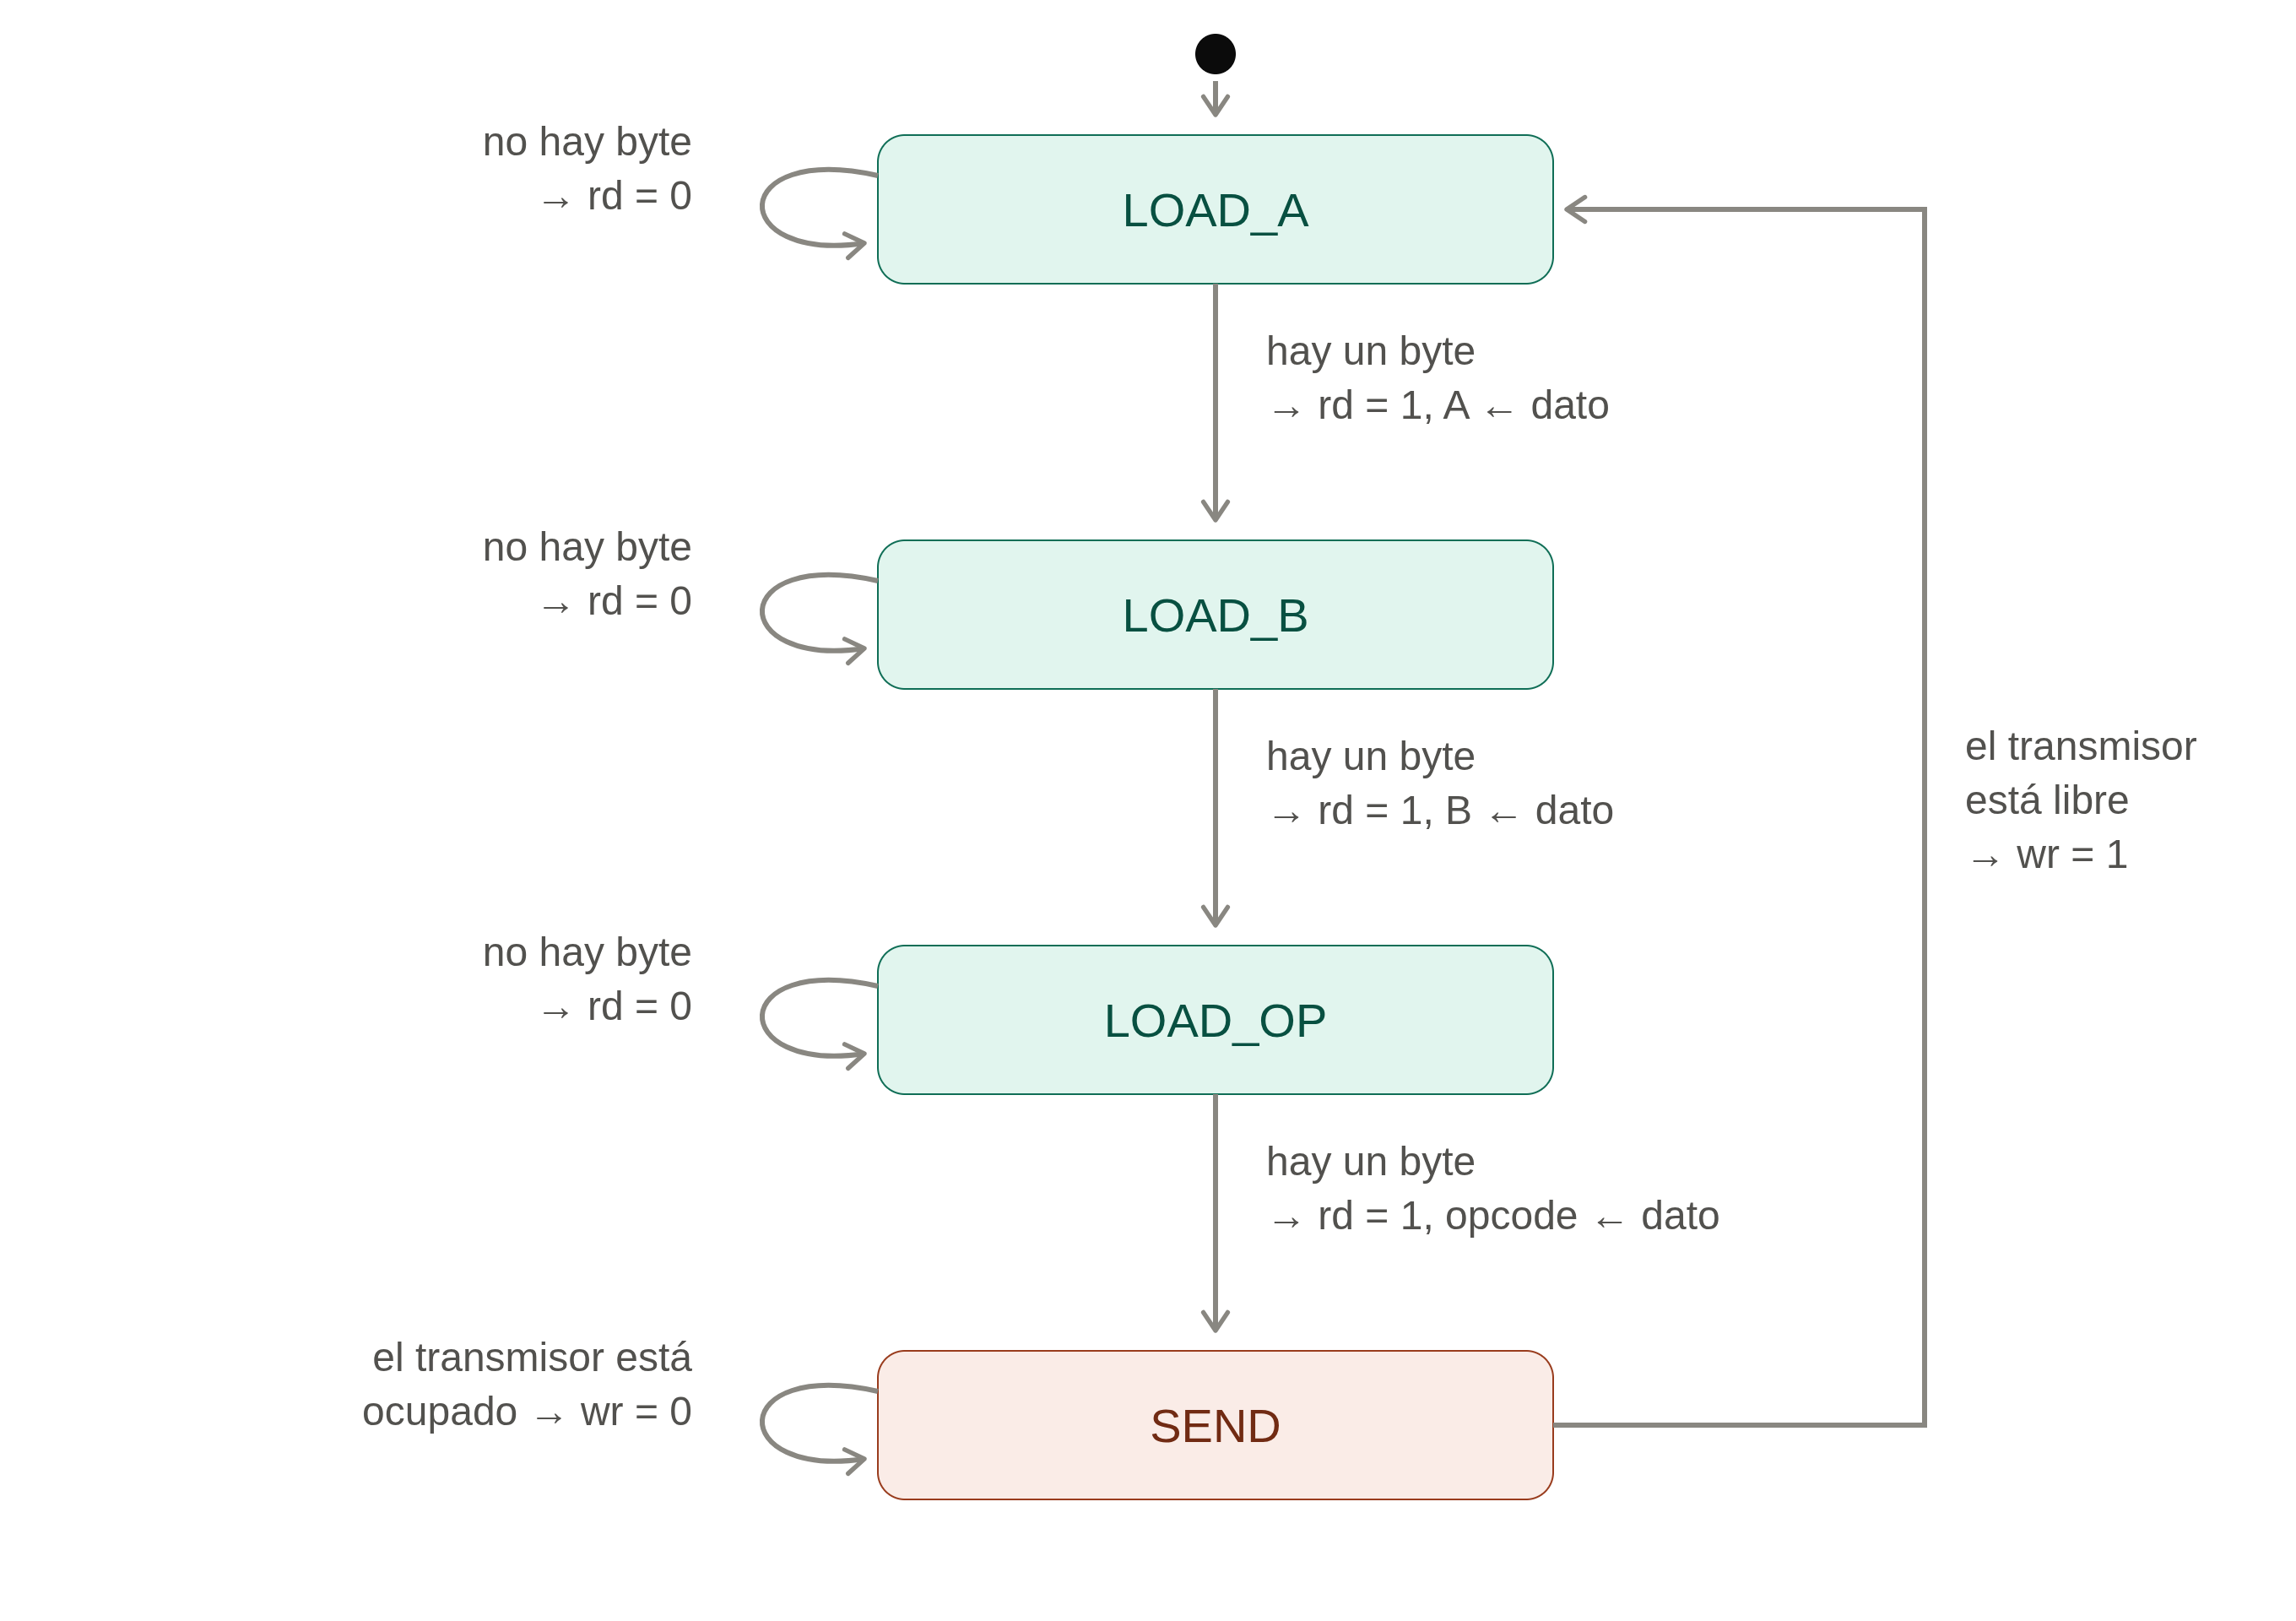
\includegraphics[width=\textwidth]{img/diagrama_estados_alu_ctrl.png}
    \caption{Diagrama de estados del control del protocolo (máquina de Mealy).}
    \label{fig:state-diagram-alu-ctrl}
\end{figure}



No fue necesario un estado de cálculo entre \texttt{LOAD\_OP} y \texttt{SEND}:
como la ALU es combinacional, en el ciclo siguiente a la carga del opcode el
resultado ya está disponible en su salida. Tampoco hizo falta un estado de
espera posterior al envío, porque el interface de transmisión retiene el dato y
la condición \texttt{tx\_full} impide escribir sobre una transmisión en curso.

\subsection{ALU}

La ALU se mantuvo tal como fue escrita en el trabajo anterior, con la única
modificación de separarla de la lógica que capturaba los operandos desde los
switches. Es puramente combinacional: no tiene reloj ni registros, y el
resultado aparece apenas se estabilizan sus entradas. Sus banderas de estado se
conectan a los LEDs de la placa.

% ============================================================
\section{Verificación}
% ============================================================

Se escribieron dos \emph{testbenches} autoverificables, que informan por consola
la cantidad de errores detectados.

\subsection{Loopback del transmisor y el receptor}

El primero conecta directamente la salida del transmisor con la entrada del
receptor, de modo que todo lo transmitido debe volver idéntico. Verifica la
cadena completa (generador de baud rate, armado de la trama y muestreo) sin
depender de la placa.

Los patrones de prueba se eligieron para cubrir los casos límite:
\texttt{0x55} y \texttt{0xAA} (bits alternados, sensibles a errores de
alineación), \texttt{0x00} (nueve bits consecutivos en 0 contando el start),
\texttt{0xFF} (datos indistinguibles de la línea en reposo) y \texttt{0x01} y
\texttt{0x80} (verifican el orden LSB primero). El testbench también comprueba
que la línea permanezca en 1 mientras el transmisor está en reposo.

\subsection{Sistema completo}

El segundo testbench instancia el módulo top completo y, del otro lado de las
líneas serie, una segunda instancia del módulo \texttt{uart} que cumple el rol de
la PC: envía los tres bytes y recibe la respuesta. Se verificaron 16 casos, que
incluyen las ocho operaciones y situaciones particulares.

\begin{table}[H]
  \centering
  \small
  \begin{tabular}{@{}lllll@{}}
    \toprule
    \textbf{Caso} & \textbf{A} & \textbf{B} & \textbf{Resultado} & \textbf{Banderas} \\
    \midrule
    ADD            & \texttt{05} & \texttt{03} & \texttt{08} & -- \\
    SUB            & \texttt{03} & \texttt{05} & \texttt{FE} & carry \\
    AND            & \texttt{0F} & \texttt{F0} & \texttt{00} & zero \\
    OR             & \texttt{0F} & \texttt{F0} & \texttt{FF} & -- \\
    XOR            & \texttt{0F} & \texttt{FF} & \texttt{F0} & -- \\
    NOR            & \texttt{0F} & \texttt{F0} & \texttt{00} & zero \\
    SRA            & \texttt{80} & \texttt{01} & \texttt{C0} & -- \\
    SRL            & \texttt{80} & \texttt{01} & \texttt{40} & -- \\
    ADD con carry  & \texttt{FF} & \texttt{01} & \texttt{00} & zero, carry \\
    ADD con overflow & \texttt{7F} & \texttt{01} & \texttt{80} & overflow \\
    Opcode inválido  & \texttt{09} & \texttt{02} & \texttt{00} & zero \\
    \bottomrule
  \end{tabular}
  \caption{Casos verificados en simulación (todos correctos).}
\end{table}

Además se comprobó que por cada operación llegue exactamente un byte de
respuesta, y que dos operaciones consecutivas sin pausa entre tramas se resuelvan
correctamente.

Para acortar los tiempos de simulación se utilizó una velocidad elevada
(\texttt{BAUD\_RATE = 1562500}, que da $N = 4$); la lógica ejercitada es la
misma, ya que lo único que cambia es cada cuántos ciclos llega el tick.

% ============================================================
\section{Implementación en la placa}
% ============================================================

\subsection{Conexión física}

La placa se conecta a la PC mediante un único cable USB que cumple tres
funciones: alimenta la placa, permite programarla por JTAG y transporta la
comunicación serie. La FPGA no maneja el protocolo USB: en la placa hay un chip
puente (FT2232HQ) que traduce entre USB y UART, de modo que el diseño solo ve
dos líneas serie comunes. Del lado de la PC, el sistema operativo crea un puerto
serie virtual.

\subsection{Asignación de pines}

\begin{table}[H]
  \centering
  \small
  \begin{tabular}{@{}llll@{}}
    \toprule
    \textbf{Puerto} & \textbf{Dirección} & \textbf{Pin} & \textbf{Función} \\
    \midrule
    \texttt{i\_clk}      & entrada & W5  & oscilador de 100~MHz \\
    \texttt{i\_reset}    & entrada & U18 & pulsador central (btnC) \\
    \texttt{i\_rx}       & entrada & B18 & línea serie desde el puente \\
    \texttt{o\_tx}       & salida  & A18 & línea serie hacia el puente \\
    \texttt{o\_leds[0]}  & salida  & U16 & bandera zero \\
    \texttt{o\_leds[1]}  & salida  & E19 & bandera carry \\
    \texttt{o\_leds[2]}  & salida  & U19 & bandera overflow \\
    \bottomrule
  \end{tabular}
  \caption{Asignación de pines (estándar LVCMOS33).}
\end{table}

Un detalle a tener en cuenta es que, en el archivo de constraints provisto por
Digilent, los nombres de los pines de la UART están puestos desde el punto de
vista del chip puente: el pin B18, identificado como \texttt{RsRx}, corresponde
a la \emph{salida} del puente y por lo tanto es la entrada de la FPGA.

\subsection{Prueba con la PC}

Para operar el sistema se desarrolló un script de Python con interfaz gráfica.
El script permite seleccionar el puerto y la velocidad, enviar los operandos y
el código de operación, y muestra el resultado en hexadecimal, decimal (con y
sin signo) y binario. Además incluye un modelo de la ALU escrito en Python, con
el que compara automáticamente la respuesta de la FPGA e indica si coincide.

\begin{figure}[H]
    \centering
    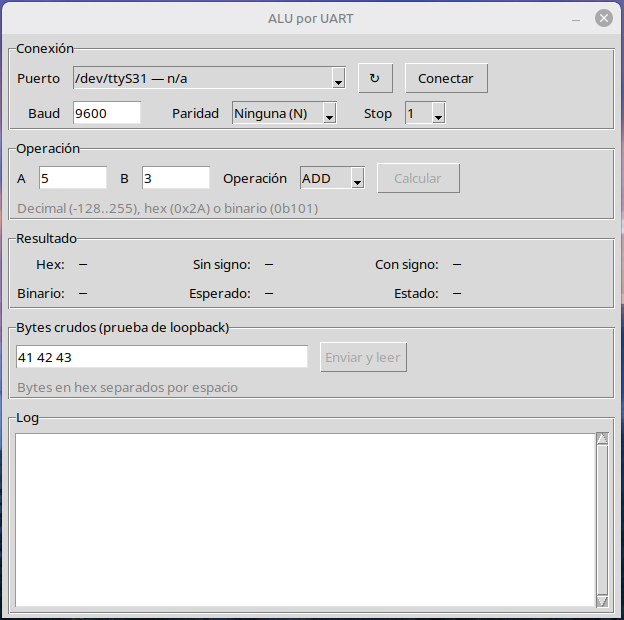
\includegraphics[width=0.7\textwidth]{img/python-script-uart.png}
    \caption{GUI del script de python utilizado}
    \label{fig:script}
\end{figure}

Una particularidad de la comunicación es que los valores deben enviarse como
\emph{bytes crudos} y no como caracteres: escribir ``5'' en una terminal
convencional transmite el código ASCII correspondiente (\texttt{0x35}) y no el
número 5. Esa es la razón por la que se optó por un script propio en lugar de
una terminal serie genérica.

% ============================================================
\section{Conclusiones}
% ============================================================

Se logró implementar una UART funcional y utilizarla para operar la ALU desde
una PC, cumpliendo con el objetivo del trabajo. El sistema fue verificado en
simulación mediante dos testbenches autoverificables y luego probado sobre la
placa.

Las principales conclusiones del desarrollo son:

\begin{itemize}[nosep]
  \item La separación entre FSM y datapath (FSMD) es lo que hace manejable el
        problema: sin ella, el receptor requeriría una cantidad inviable de
        estados.
  \item La señal del generador de baud rate debe usarse como habilitación y
        nunca como reloj, para no generar relojes derivados de lógica.
  \item Toda señal proveniente del exterior necesita un sincronizador de dos
        flip-flops antes de entrar a la lógica, ya que de lo contrario distintos
        registros pueden leer valores distintos en el mismo ciclo.
  \item El patrón de \emph{dato más bandera de validez} se repite en cada
        frontera del sistema y es lo que permite que módulos con tiempos muy
        distintos (una trama dura unos $10^5$ ciclos de reloj, un pulso dura uno)
        trabajen juntos sin perder información.
  \item Definir interfaces angostas y estables entre módulos permitió reutilizar
        la ALU del trabajo anterior sin modificar una sola línea de su lógica.
\end{itemize}

Como posibles mejoras quedan pendientes el agregado de bit de paridad y
detección de errores de trama, y un protocolo con byte de sincronismo: al ser
posicional, si se pierde o se cuela un byte la máquina de control queda desfasada
y es necesario reiniciarla con el pulsador de reset.

% ============================================================
\begin{thebibliography}{9}
\bibitem{chu}
P.~P. Chu, \emph{FPGA Prototyping by Verilog Examples: Xilinx Spartan-3 Version}.
Wiley, 2008.

\bibitem{basys3}
Digilent, \emph{Basys 3 FPGA Board Reference Manual}, 2016.

\bibitem{xdc}
Digilent, \emph{Basys-3-Master.xdc}, repositorio \texttt{digilent-xdc},
\url{https://github.com/Digilent/digilent-xdc}.

\bibitem{catedra}
Cátedra de Arquitectura de Computadoras, \emph{Máquinas de Estado Finitas --
TP: UART}, FCEFyN, UNC.
\end{thebibliography}

\end{document}